\subsection{Visione}

\subsubsection{Cronologia revisioni}


\begin{table}[htb]
	\begin{tabular}{|l|l|l|l|}
		\hline
		
		\textbf{Versione} & \textbf{Data}       & \textbf{Descrizione} & \textbf{Autore}           \\ \hline
		
		1.0      & 14/02/2019 & Prima bozza & Pietro Mazzaglia \\ \hline
		1.1      & 16/02/2019 & Revisione a fine Ideazione & Pietro Mazzaglia \\ \hline
		1.2      & 21/02/2019 & Revisione a fine Iterazione 1 & Pietro Mazzaglia \\ \hline
		1.3      & 24/02/2019 & Revisione a fine Iterazione 2 & Pietro Mazzaglia \\ \hline
		1.4      & 01/03/2019 & Revisione a fine Iterazione 4 & Pietro Mazzaglia \\ \hline		
	\end{tabular}
\end{table}

\subsubsection{Introduzione}

Il progetto in questione ambisce a garantire funzionalità su più livelli per la gestione della vita all'interno di un Campus universitario. 

La piattaforma \textit{uCOM} vuole essere flessibile, per l'aggiunta di funzionalità ulteriori e per adattarsi all'utilizzo presso strutture diverse. 

Il sistema software deve prestarsi all'interazione con altri sistemi esterni, per la gestione dei servizi relativi.

\subsubsection{Posizionamento}

\underline{\textit{Opportunità di business}}

Attualmente la scelta di vivere in residenze e alloggi comuni è la scelta più frequente per gli studenti che scelgono di studiare in una città diversa da quella di provenienza.

Spesso tali residenze non si limitano ad offrire servizi di alloggio, bensì garantiscono anche servizi di ristorazione o altri servizi accessori, come palestre, biblioteche, e la possibilità di frequentare corsi e seminari all'interno della struttura.

Il committente di questo progetto è un'entità di questo genere, tuttavia lo sviluppo di un software flessibile rappresenta un'opportunità per imporsi nel settore di riferimento, oltre che per soddisfare la commissione del cliente.

\underline{\textit{Formulazione del problema}}

Nonostante la diffusione del modello di residenza descritto, non esiste una piattaforma comune e di semplice utilizzo che tali strutture possano adottare per automatizzare la gestione interna, dunque spesso non vengono forniti strumenti che supportino gli usufruitori dei servizi, e molte mansioni sono svolte manualmente.

Inoltre è raro che applicazioni di questo tipo siano progettate in maniera flessibile, tale da adattarsi ad eventuali estensioni di funzionalità o alla collaborazione con servizi forniti esternamente.

\underline{\textit{Formulazione del posizionamento del prodotto}}

\textit{uCOM} potrebbe garantire un sistema semplice da utilizzare, affidabile e ricco di funzionalità, per la gestione di un Campus. 

L'utilizzo di una piattaforma unica rappresenta un vantaggio anche per gli utenti, che necessitano di imparare ad utilizzare un solo software, anche nel caso in cui decidano di cambiare Campus o città.

La scelta di affidarsi a un servizio esterno inoltre solleverebbe le strutture dai costi ingenti relativi allo sviluppo di un software proprietario.

\underline{\textit{Alternative e concorrenza}}

Alcuni campus possiedono applicazioni esclusive per la gestione della propria struttura, tuttavia una soluzione di questo tipo non è considerabile longeva. Aggiornamento e mantenimento di un prodotto \textit{custom} comportano spese elevate che non tutti gli enti sono pronti a sostenere.

Una piattaforma comune che venga continuamente aggiornata e supportata da un'azienda che sviluppi software, quale \textit{uCOM}, rappresenta la strada giusta per garantire maggiore longevità al proprio prodotto.

Concorrenti:
\begin{itemize}
	\item GuideBook Edu [\url{https://guidebook.com/schools/}]
	\item Applicazioni proprietarie dei singoli Campus
\end{itemize}

\newpage

\subsubsection{Descrizione delle parti interessate}

\underline{\textit{Dati demografici di mercato}}

Secondo un report UNESCO
\footnote{Report: \url{https://unesdoc.unesco.org/ark:/48223/pf0000247862}} 
nel 2014 erano 207 milioni gli studenti universitari nel mondo, e secondo i trend recenti tale numero non può che essere aumentato.

Il numero di Campus è direttamente proporzionale a quello degli studenti.

\underline{\textit{Riepilogo delle parti interessate}}

% Please add the following required packages to your document preamble:
% \usepackage{graphicx}
\begin{table}[!htb]
	\resizebox{\textwidth}{!}{%
		\begin{tabular}{|l|l|l|}
			\hline
			\textbf{Nome}                                                           & \textbf{Descrizione}                                                                                                                  & \textbf{Responsabilità}                                                                                                                                                                                                             \\ \hline
			\begin{tabular}[c]{@{}l@{}}Team di sviluppo\\ del software\end{tabular} & \begin{tabular}[c]{@{}l@{}}Responsabile dello\\ sviluppo software\end{tabular}                                                        & \begin{tabular}[c]{@{}l@{}}Design e implementazione\\ del progetto.\\ \\ Deve garantire standard di\\ qualità e affidabilità.\end{tabular}                                                                                                                                                     \\ \hline
			Direzione del Campus                                                    & \begin{tabular}[c]{@{}l@{}}Committente del progetto\\ e gestore della struttura\\ per cui l'applicazione è \\ progettata\end{tabular} & \begin{tabular}[c]{@{}l@{}}Richiede che il software \\ soddisfi i requisiti funzionali\\ per il corretto svolgimento di\\ ogni operazione e \\ che siano soddisfatti i requisiti\\ di qualità (non funzionali)\end{tabular} \\ \hline
			Fornitori di servizi                                                    & \begin{tabular}[c]{@{}l@{}}I fornitori di servizi del\\ Campus, quali mensa,\\ biblioteca, ...\end{tabular}                           & \begin{tabular}[c]{@{}l@{}}Permettere l'integrazione o \\ l'interazione tramite \\ un'interfaccia del proprio \\ servizio attraverso la piattaforma.\end{tabular}                                                                                         \\ \hline
		\end{tabular}%
	}
\end{table}

\underline{\textit{Riepilogo dell'utente}}

Gli utilizzatori dell'applicazione sono:

\begin{itemize}
	\item \textbf{Studenti :}  utilizzano la piattaforma per accedere ai servizi del Campus e comunicare con l'amministrazione
	\item \textbf{Amministratori :} utilizzano la piattaforma per gestire i servizi del Campus e comunicare con gli Studenti
	\item \textbf{System Admin :}  utilizzano la piattaforma per gestire gli utenti e mantenere un certo livello di sicurezza del sistema
\end{itemize}

\newpage

\underline{\textit{Obiettivi delle parti interessate}}

% Please add the following required packages to your document preamble:
% \usepackage{graphicx}
\begin{table}[!htb]
	\resizebox{\textwidth}{!}{%
		\begin{tabular}{|l|l|l|l|}
			\hline
			\textbf{\begin{tabular}[c]{@{}l@{}}Obiettivi di \\ alto livello\end{tabular}} & \textbf{Priorità} & \textbf{Problemi}                                                                                                                                                                                                                                                                                                                                                                                                                                                                                  & \textbf{Soluzioni attuali}                                                                                                                                                                                                                                                                                   \\ \hline
			Flessibilità                                                                  & alta             & \begin{tabular}[c]{@{}l@{}}Necessità di ampliare le funzionalità dell'applicazione\\ per adeguarle ai servizi offerti dalle strutture.\end{tabular}                                                                                                                                                                                                                                                                                                                                                & \begin{tabular}[c]{@{}l@{}}Le attuali soluzioni sono \\ poco flessibili e il loro ampliamento\\ comporta enormi sforzi di sviluppo.\end{tabular}                                                                                                                                                             \\ \hline
			Automatizzazione                                                              & alta              & \begin{tabular}[c]{@{}l@{}}La mancanza di servizi di automatizzazione rallenta \\ le operazioni di gestione dei servizi di un Campus.\\ \\Un sistema automatizzato permette una maggiore interazione \\ tra Studenti e Amministrazione, con uno sforzo minore, da\\ entrambe le parti.\end{tabular} & \begin{tabular}[c]{@{}l@{}}Alcune strutture scelgono di sviluppare\\ o di acquistare software personalizzato, \\ spendendo ingenti cifre di denaro\end{tabular}
			\\ \hline
			Affidabilità                                                                  & alta              & \begin{tabular}[c]{@{}l@{}}Le operazioni devono essere gestite in maniera sicura e affidabile.\\ \\ Il sistema deve garantire la corretta fruizione dei servizi e un \\ canale di comunicazione sicuro e affidabile.\end{tabular}                                                                                                                                                                                                                                                                  & \begin{tabular}[c]{@{}l@{}}Le attuali soluzioni non automatizzate \\ non sono in grado di garantire un alto \\ grado di affidabilità.\\ \\ Piattaforme personalizzate possono\\ risentire di bug più frequentemente \\ rispetto a un progetto unico che è\\ testato e utilizzato su larga scala\end{tabular} \\ \hline
			
			Integrazione                                                                 & alta              & \begin{tabular}[c]{@{}l@{}} Il sistema deve fornire ai servizi esterni dati coerenti con le\\ loro piattaforme.\end{tabular}                                                                                                                                                                                                                                                                  & \begin{tabular}[c]{@{}l@{}}Nessuna.\end{tabular} 
			\\ \hline
			Portabilità                                                              & media              & \begin{tabular}[c]{@{}l@{}}Necessità di una piattaforma che sia disponibile\\ sia su smartphone, che su computer.\end{tabular} & \begin{tabular}[c]{@{}l@{}}Nessuna\end{tabular}                                                                                                                                                                                                                                                                                            \\ \hline
			Semplicità                                                                    & media              & \begin{tabular}[c]{@{}l@{}}E' necessario che l'applicazione sia semplice da utilizzare e \\ progettata secondo un formato che gli utenti conoscano bene e\\ a cui sono abituati.\end{tabular}                                                                                                                                                                                                                                                                                                      & \begin{tabular}[c]{@{}l@{}}La gestione manuale o senza\\ un'applicazione predefinita comporta\\ difficoltà d'uso per gli utenti.\end{tabular}           \\ \hline                                                                                                                                                     
		\end{tabular}%
	}
\end{table}

\underline{\textit{Obiettivi degli utenti}}

\begin{itemize}
	\item \textbf{Studente :} prenotare pasti mensa, richiedere prestiti
	biblioteca, iscriversi ai corsi, comunicare con l'amministrazione
	\item \textbf{Amministratore :} gestire corsi, gestire iscrizioni ai corsi, comunicare con gli studenti
	\item \textbf{System Admin :} gestire utenti
\end{itemize}

\newpage

\subsubsection{Descrizione generale del prodotto}

\underline{\textit{Punto di vista del prodotto}}

La piattaforma \textit{uCOM} sarà disponibile su computer desktop e laptop, e dispositivi mobili per essere facilmente utilizzabile sia dall'amministrazione che dagli studenti.

Esso fornirà servizi agli utenti e collaborerà con altri sistemi come indicato in figura.

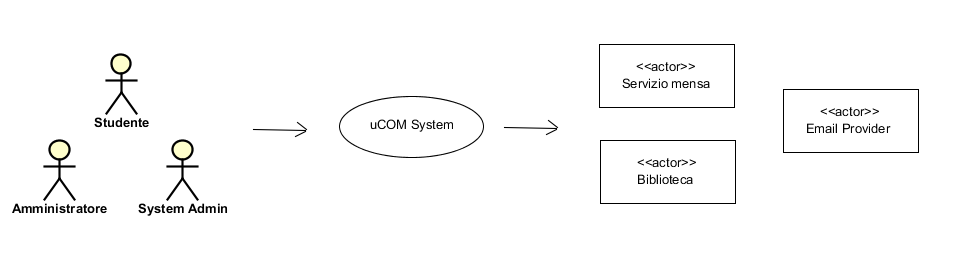
\includegraphics[scale = 0.8]{context_diagram.png}

\underline{\textit{Sintesi dei benefici}}

% Please add the following required packages to your document preamble:
% \usepackage{graphicx}
\begin{table}[!htb]
	\resizebox{\textwidth}{!}{%
		\begin{tabular}{|l|l|}
			\hline
			\textbf{Funzionalità supportata}                                                                                                        & \textbf{Beneficio della parte interessata}                                                                                                                                                                \\ \hline
			\begin{tabular}[c]{@{}l@{}}Funzionalmente, il sistema fornisce\\ diversi servizi comuni per la gestione\\ di un Campus\end{tabular}     & \begin{tabular}[c]{@{}l@{}}La Direzione del Campus mette a \\ disposizione un servizio veloce, affidabile\\ e semplice da utilizzare\end{tabular}                                                         \\ \hline
			\begin{tabular}[c]{@{}l@{}}Sistema di comunicazione, facilmente\\ accessibile e sicuro\end{tabular}                                     & \begin{tabular}[c]{@{}l@{}}Gli utenti beneficiano di un mezzo di\\ comunicazione telematico che permette\\ maggiore rapidità nelle interazioni\end{tabular}                                             \\ \hline
			\begin{tabular}[c]{@{}l@{}}Flessibile per l'aggiunta di nuove\\ funzionalità e per l'applicazione di \\ regole di business\end{tabular} & \begin{tabular}[c]{@{}l@{}}La Direzione del Campus può decidere\\ di variare i contratti con i propri fornitori\\ di servizi, senza dover mutare la \\ piattaforma su cui si appoggia (\textit{uCOM})\end{tabular} \\ \hline
		\end{tabular}%
	}
\end{table}

\underline{\textit{Ipotesi e dipendenze}}

\begin{itemize}
	\item Si suppone  che un servizio di accesso alla rete internet sia disponibile (in circostanze di utilizzo normali)
	\item Si suppone che i dispositivi permettano l'installazione di software multipiattaforma
\end{itemize}

\newpage

\underline{\textit{Prezzi}}

Il software sarà venduto ad ogni Campus con pagamento su base mensile. L'ammontare della rata è definito dal numero di utenti attivi che il Campus registra durante il mese.

\underline{\textit{Licenze e installazioni}}

Il software verrà rilasciato sotto licenza EULA.

\subsubsection{Riepilogo delle caratteristiche di sistema}

\begin{itemize}
	\item Utilizzo dei servizi interni del Campus
	\item Interfaccia con i servizi esterni forniti al Campus
	\item Gestione degli errori, attraverso notifica all'utente e tentativo di risoluzione
	\item Possibilità di estensione delle funzionalità
	\item Possibilità di adeguamento dei sistemi esterni coinvolti
	\item Servizio distribuito tramite rete Internet
	\item Applicazione portatile su più dispositivi
	\item Piattaforma adeguata per utenti con disabilità
\end{itemize}

\subsubsection{Altri requisiti e vincoli}

Si veda il documento delle \textit{Specifiche Supplementari} per ulteriori requisiti del progetto.











